\section{Accessing ManeFrame II (M2)}

\begin{frame}{Accessing ManeFrame II (M2)}
\begin{description}
\item[SSH]
\begin{itemize}
  \item Provides secure command line access to the login nodes.
  \item Graphical applications require X11-forwarding.
  \item Five login nodes all accessible via \mintinline{sh}{m2.smu.edu}.
  \item \href{https://s2.smu.edu/hpc/documentation/access.html}{M2 SSH Instructions}
\end{itemize}
\item[HPC Portal]
\begin{itemize}
  \item Provides web-based access to M2.
  \begin{itemize}
    \item File access
    \item Terminal access
    \item JupyterLab (Notebooks)
    \item RStudio
    \item Remote Desktops
  \end{itemize}
\end{itemize}
\item[SFTP]
\begin{itemize}
  \item Transfer files to and from M2 using an SFTP client.
  \item \href{https://s2.smu.edu/hpc/documentation/access.html}{M2 SFTP Instructions}
\end{itemize}
\end{description}
\end{frame}

\begin{frame}{ManeFrame II (M2) HPC OnDemand Web Portal}
\begin{columns}[c]
\begin{column}{0.5\textwidth}
\begin{itemize}
\item Provides an integrated single access point for HPC resources on the
ManeFrame II (M2) supercomputer
\item Accessing the Portal:
\begin{itemize}
\item Access to the HPC portal requires an existing M2 account
\item Go to \url{hpc.smu.edu}
\item Sign in using your SMU ID and SMU password
\end{itemize}
\item \href{https://s2.smu.edu/hpc/documentation/portal.html}{HPC Portal
Documentation}
\item
\href{https://s2.smu.edu/hpc/documentation/portal.html\#remote-desktop}{HPC
Portal Walkthrough Video}
\end{itemize}
\end{column}
\begin{column}{0.5\textwidth}
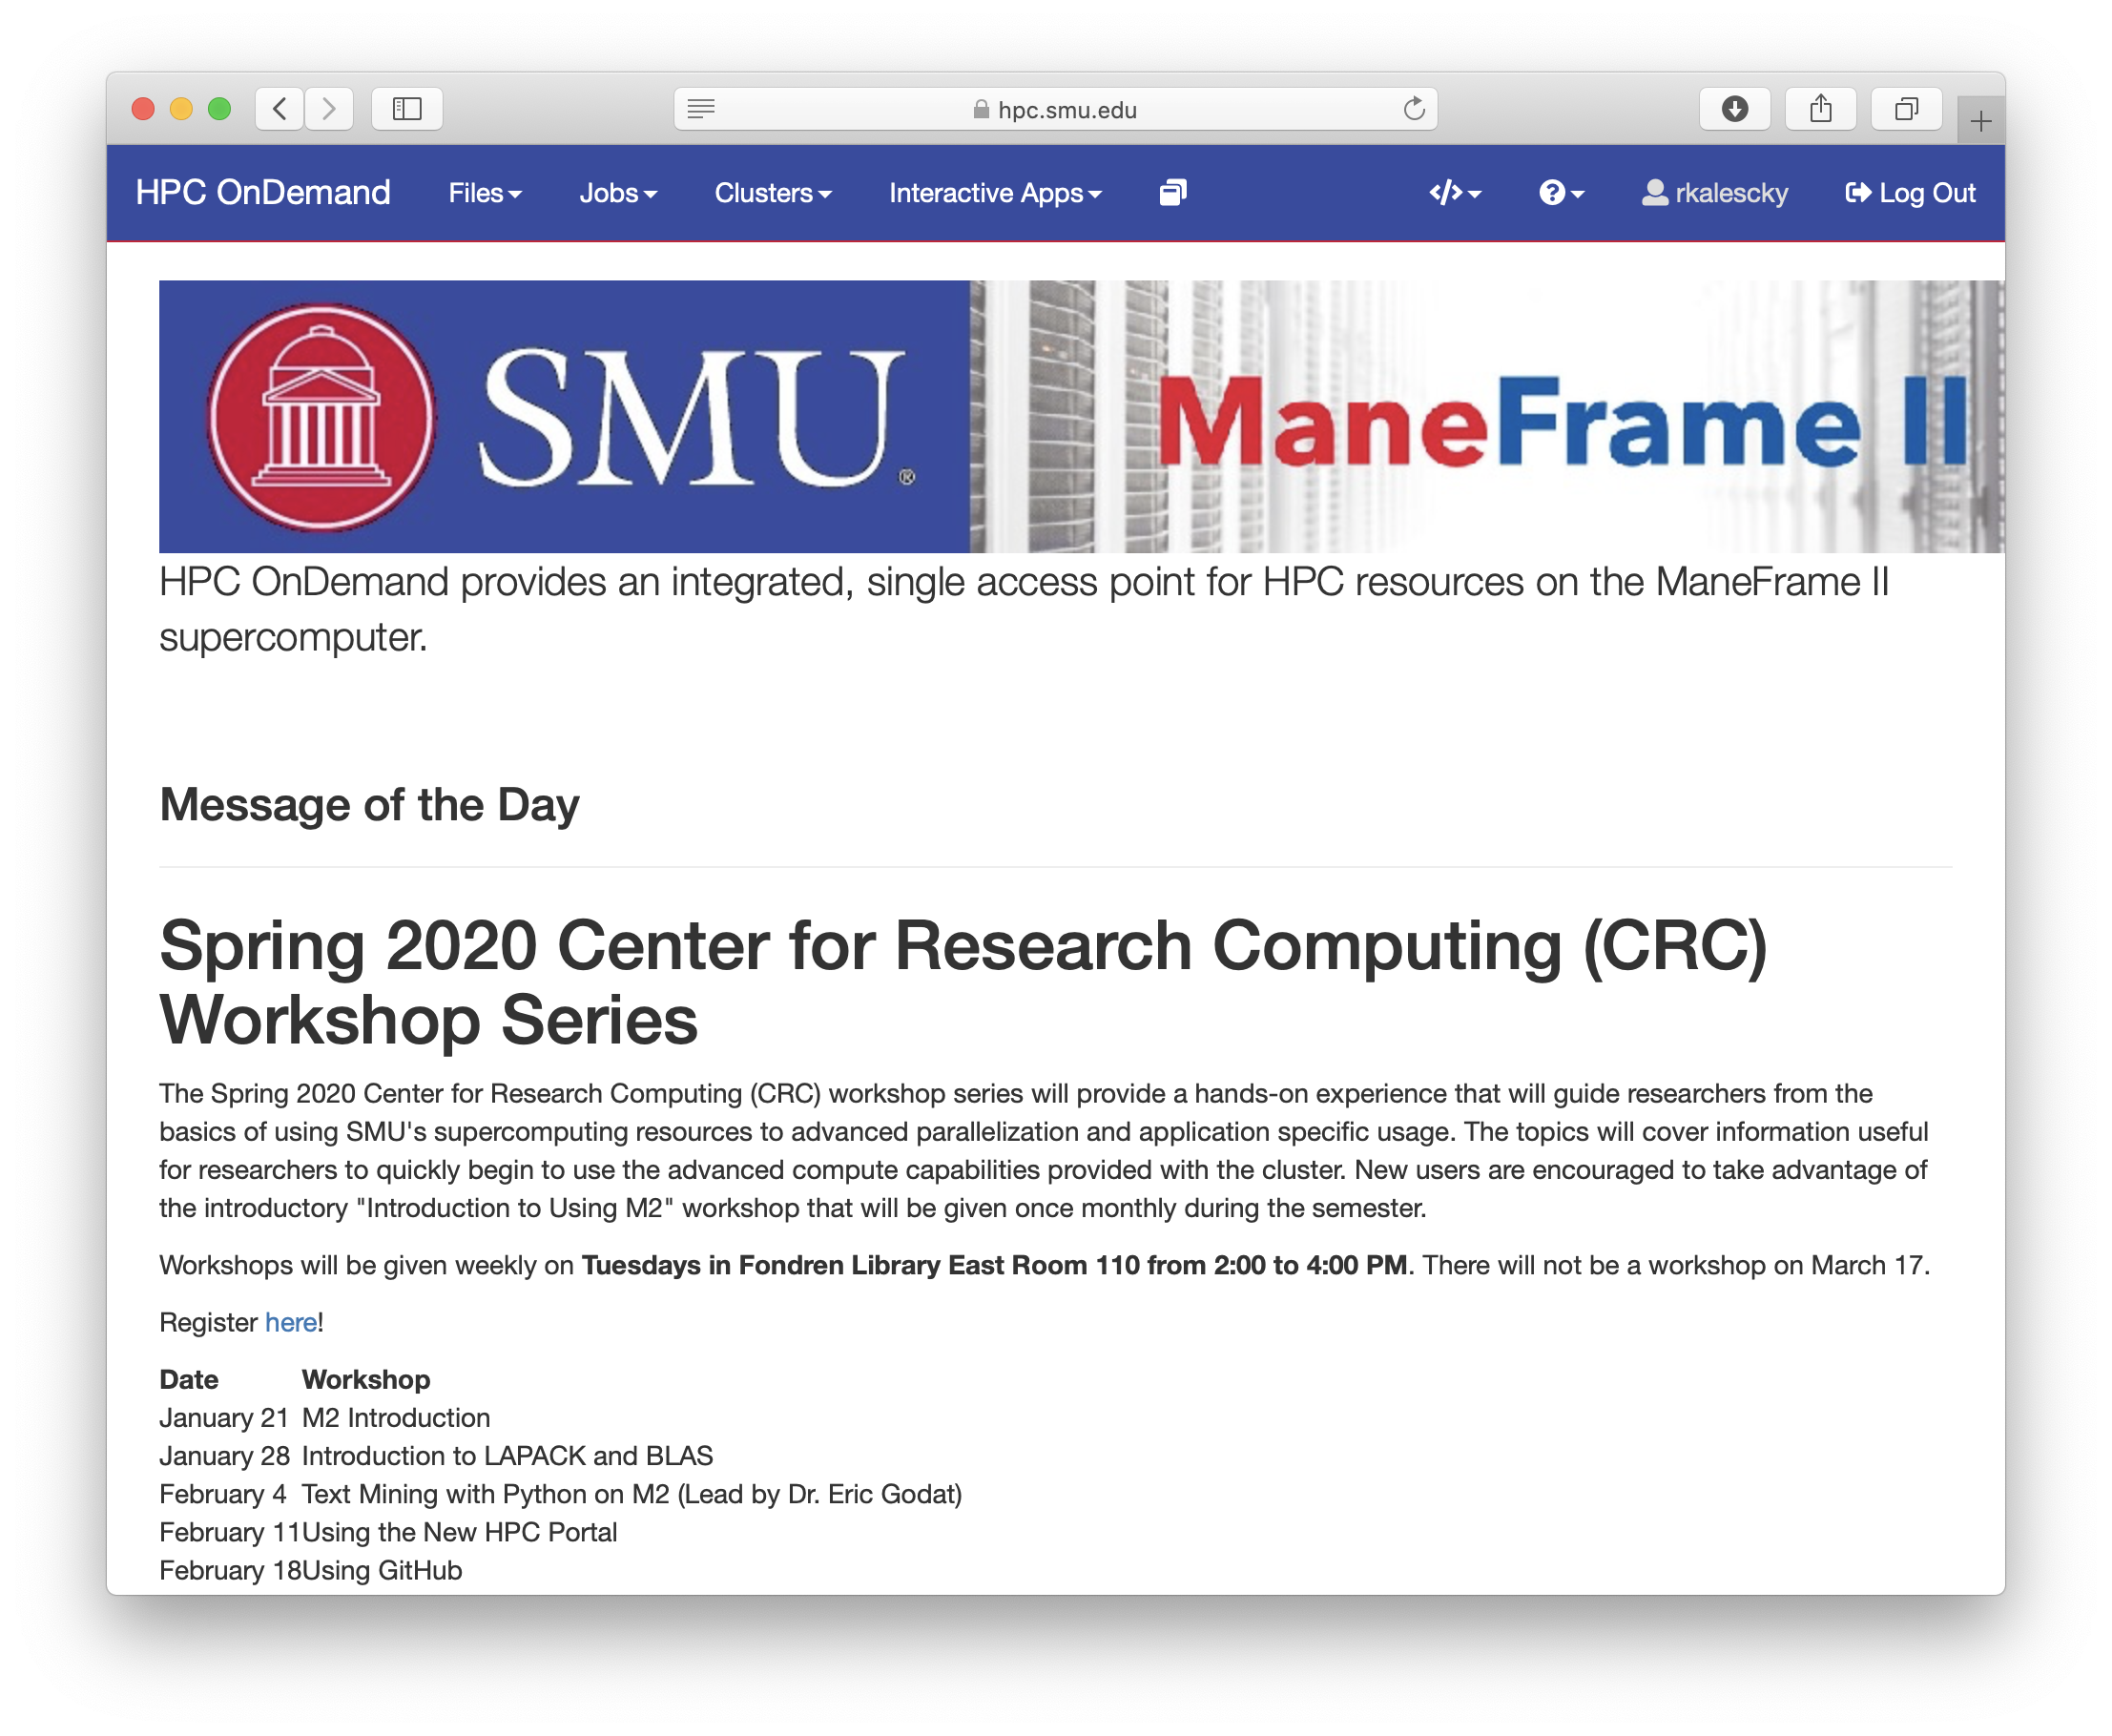
\includegraphics[width=\linewidth]{figures/portal.png}
\end{column}
\end{columns}
\end{frame}

